\begin{figure*}[h]
  \subfloat{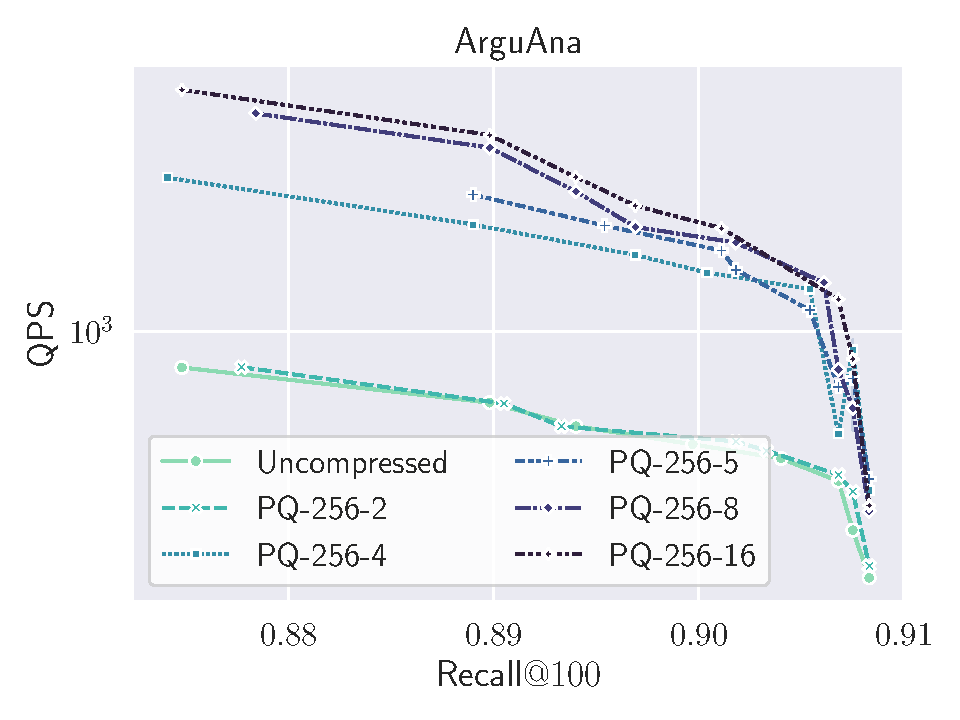
\includegraphics[width=.33\textwidth]{plots/pq_vs_qps_100/arguana-pq_vs_nopq.pdf}}
  \subfloat{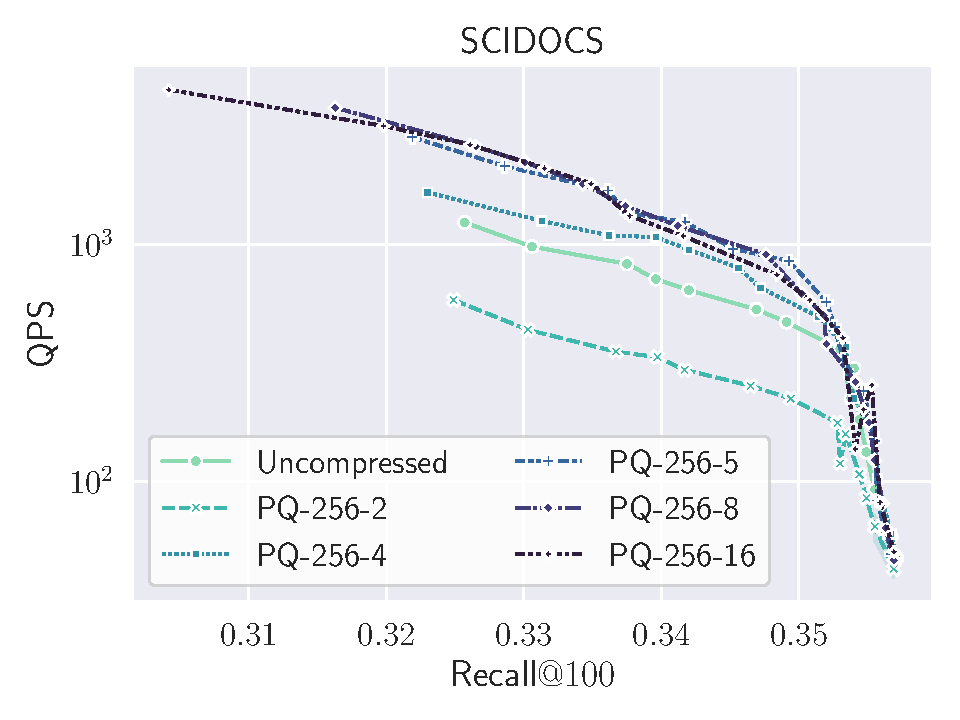
\includegraphics[width=.33\textwidth]{plots/pq_vs_qps_100/scidocs-pq_vs_nopq.pdf}}
  \subfloat{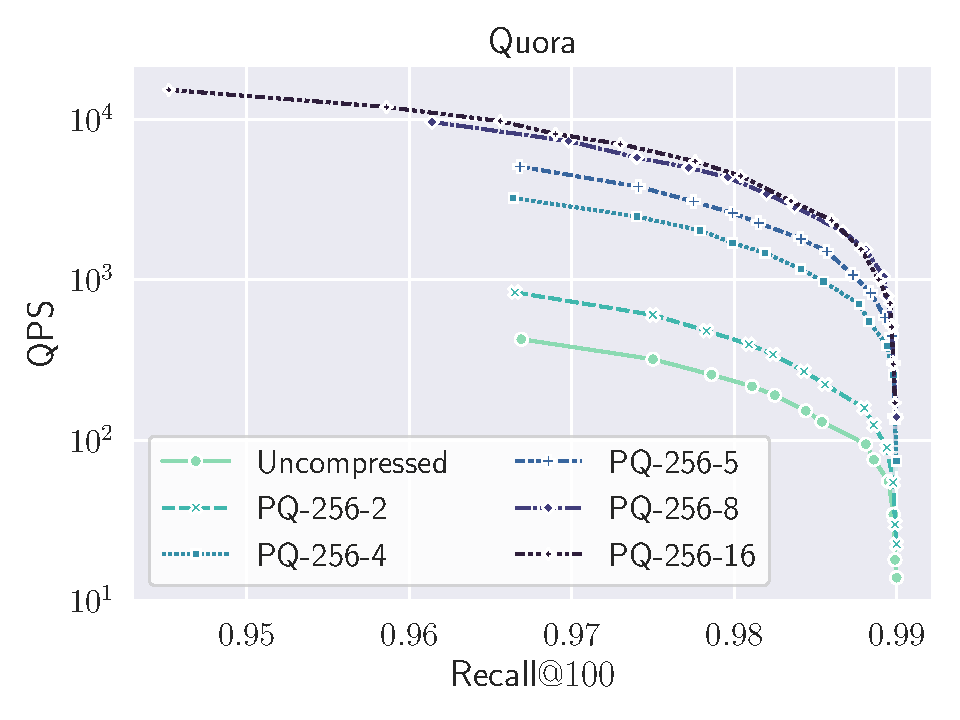
\includegraphics[width=.33\textwidth]{plots/pq_vs_qps_100/quora-pq_vs_nopq.pdf}}
  
  \subfloat{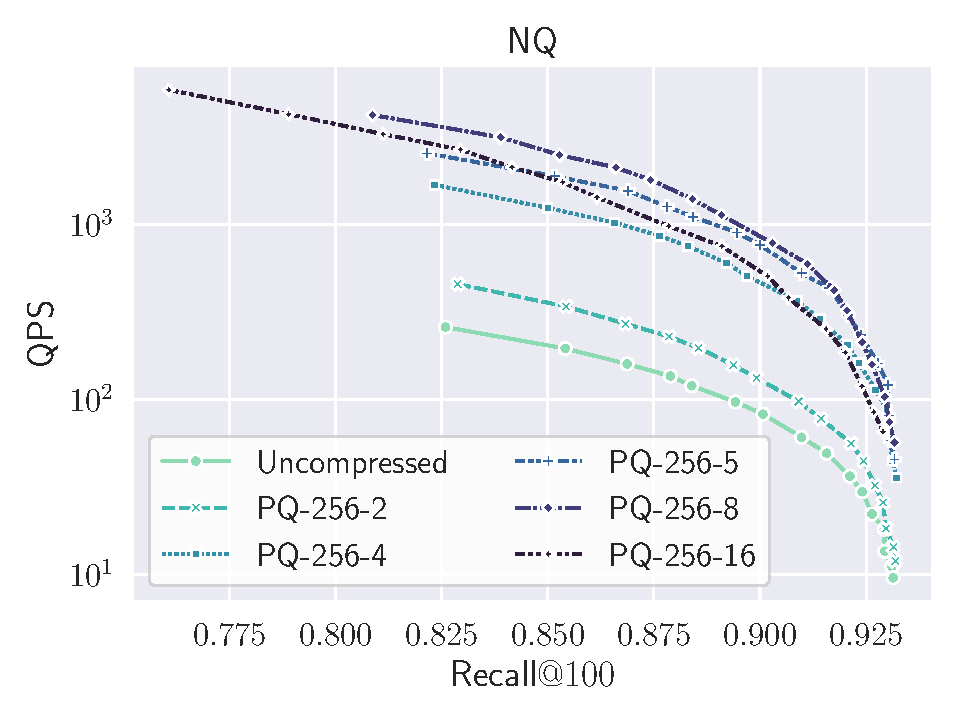
\includegraphics[width=.33\textwidth]{plots/pq_vs_qps_100/nq-pq_vs_nopq.pdf}}
  \subfloat{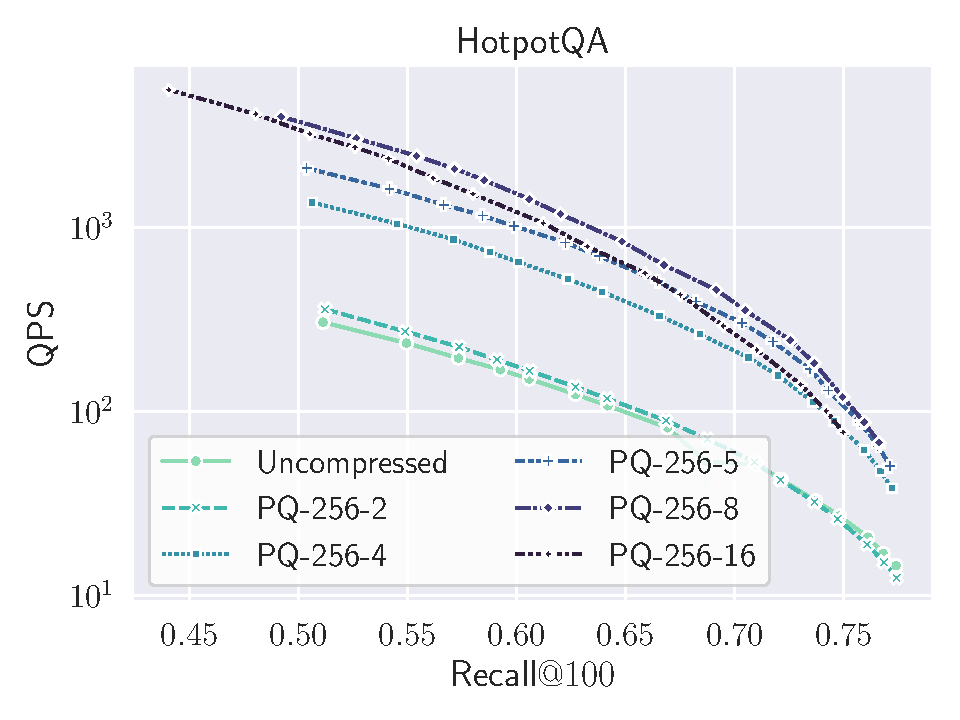
\includegraphics[width=.33\textwidth]{plots/pq_vs_qps_100/hotpotqa-pq_vs_nopq.pdf}}
  \subfloat{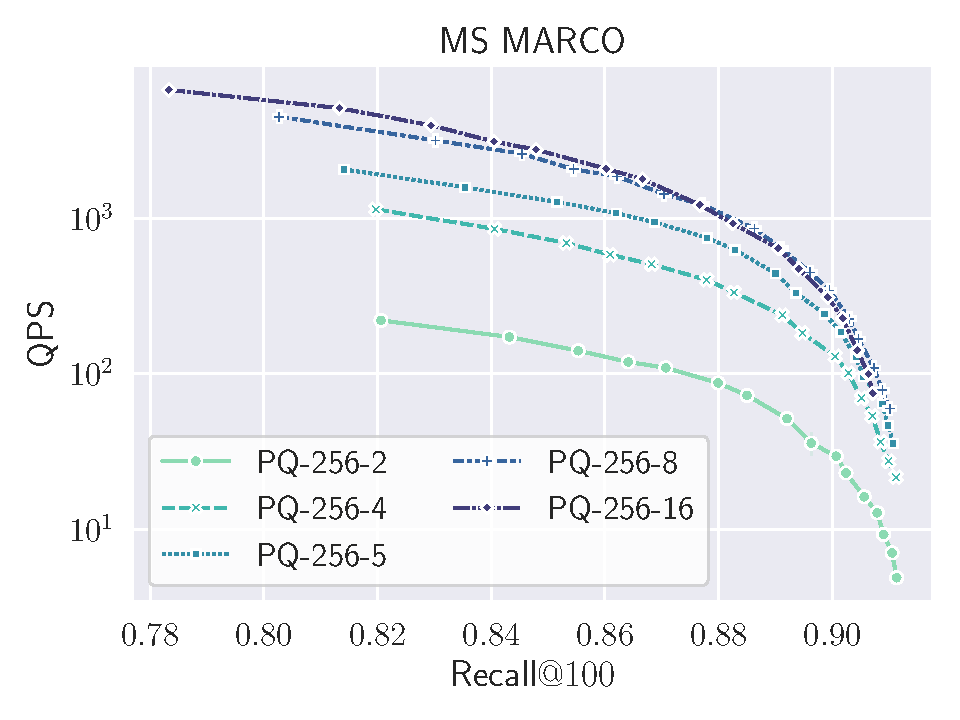
\includegraphics[width=.33\textwidth]{plots/pq_vs_qps_100/msmarco-pq_vs_nopq.pdf}}
  
\vspace{1em}
  \caption{\small Plots showing the QPS vs. Recall@$100$ for \name{} on the BEIR datasets we evaluate in this paper. The different curves are obtained by using different PQ methods on 10240-dimensional FDEs.}
\label{pq-qps-100-full}
\end{figure*}